%!TEX root = ../thesis.tex

\section{関連研究}
は,カメラ画像とステアリングの角度を教師信号とし,end-to-end学習することで自動車の自動運転に成功している.このシステムは,人間からの最小限の学習データで,車線のあるなしを問わず一般道や高速道路での渋滞中の走行を学習する.また,駐車場や未舗装路など,視覚ガイダンスが不明瞭な場所でも運転することができます.本システムは,人間の操舵角のみを学習信号として,道路の特徴を検出するなどの必要な処理を内部表現として自動的に学習させる.
     \begin{figure}[h]
          \centering
          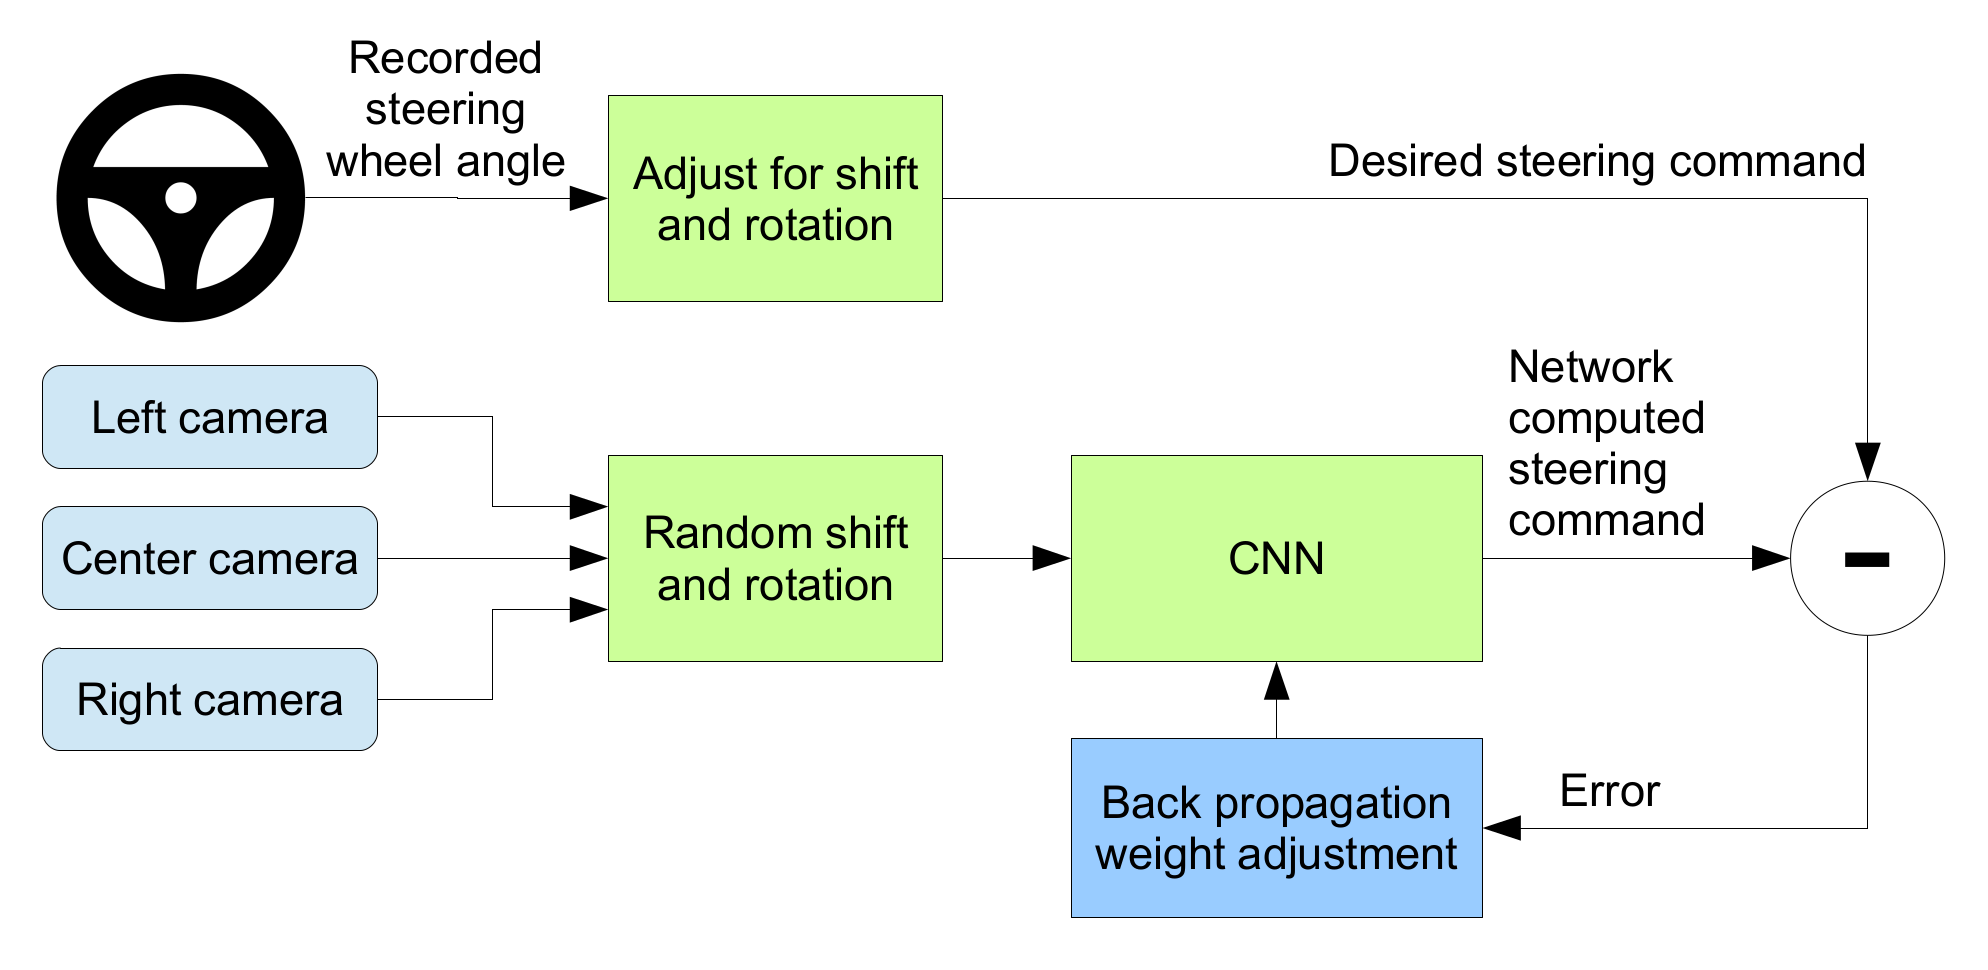
\includegraphics[keepaspectratio, scale=0.16] {images/bojarski_train.png}
          \caption{Training the neural network \cite{bojarski}}
          \label{Fig:bojarski_train}
     \end{figure}

学習後は,\figref{Fig:bojarski_test}に示すようにカメラ画像から直接,ステアリングコマンドを出力するシステムになっている.

     \begin{figure}[h]
          \centering
          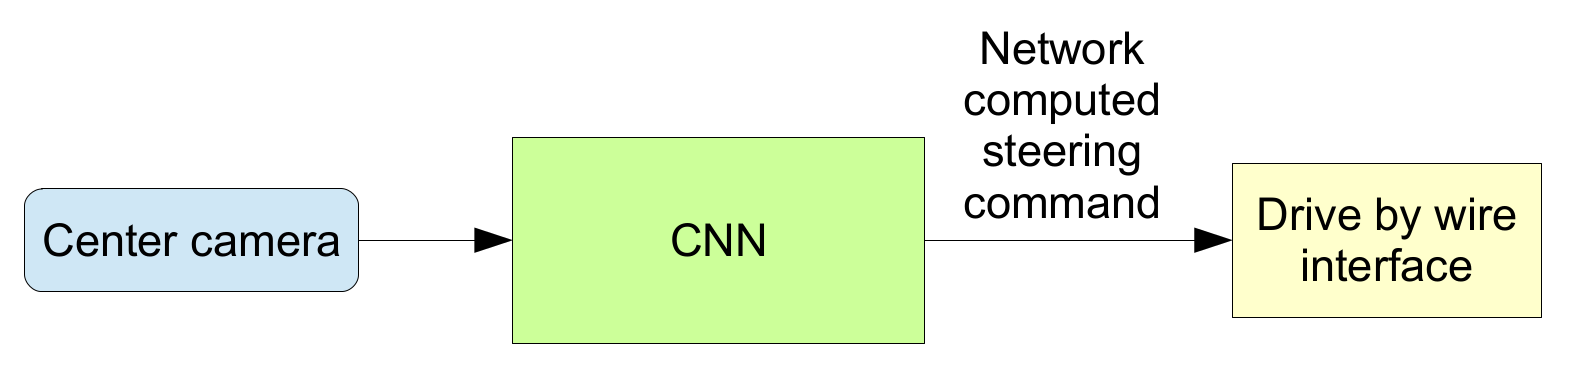
\includegraphics[keepaspectratio, scale=0.20] {images/bojarski_test.png}
          \captionsetup{justification=raggedright} % キャプションを左寄せに
          \caption{The trained network is used to generate steering commands from a single front-facing center camera. \cite{bojarski}}
          \label{Fig:bojarski_test}
     \end{figure}

このため,例えば,道路の外周を検出するような明示的な学習は行っていない.
     \begin{figure}[h]
          \centering
          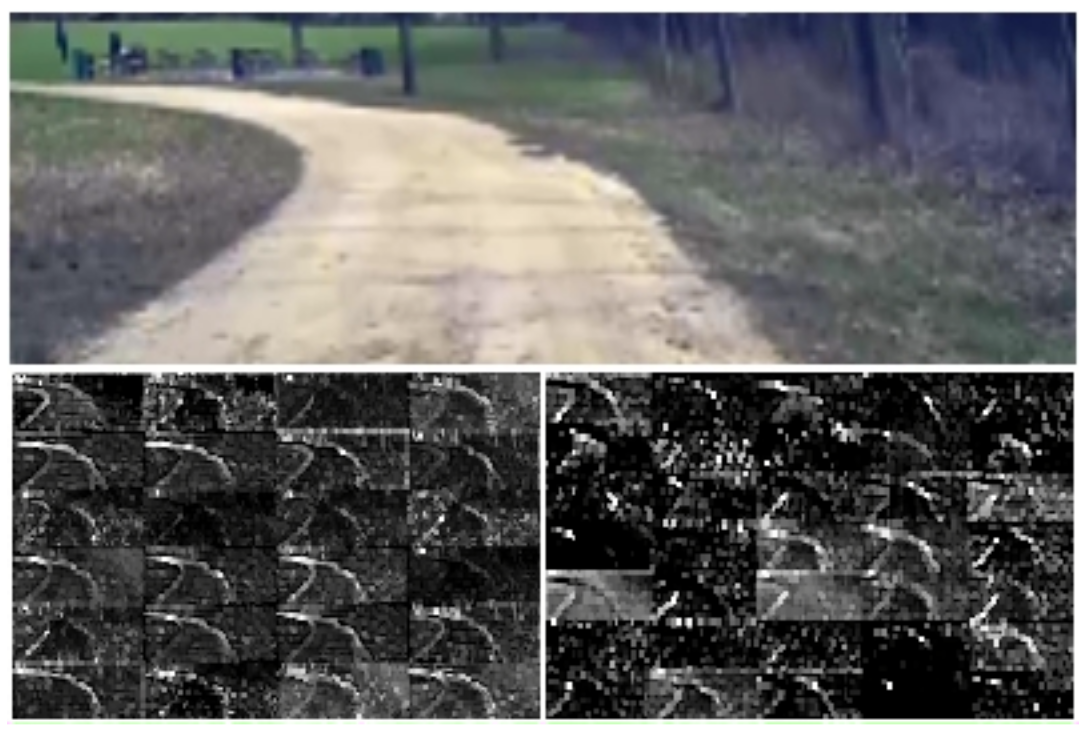
\includegraphics[keepaspectratio, scale=0.35] {images/bojarski_CNN.png}
          \captionsetup{justification=raggedright} % キャプションを左寄せに
          \caption{How the CNN ``sees'' an unpaved road. Top: subset of the camera image sent to the CNN. Bottom left: Activation of the first layer feature maps. Bottom right: Activation of the second layer feature maps. This demonstrates that the CNN learned to detect useful road features on its own, i.e., with only the human steering angle as training signal. We never explicitly trained it to detect the outlines of roads. \cite{bojarski}}
          \label{Fig:bojarski_CNN}
     \end{figure}
\newpage
